\chapter{Framework}\label{ch:framework}
This chapter serves as a way to introduce the tools that have been employed during the development of this project. All of them are \textbf{open-source}. The transparency provided by the open-source platforms is a major advantage, because the software can be joined together and adapted to our specific applications, which is mainly written in \textbf{Python} \footnote{\url{https://www.python.org/}}.

\section{JdeRobot}\label{sec:jderobot}
\textbf{JdeRobot} \footnote{\url{http://jderobot.org}} is an open source middleware for robotics and computer vision. It has been designed to simplify the software development within these fields. It's mostly written in C\nolinebreak[4]\hspace{-.05em}\raisebox{.4ex}{\tiny\bf ++} language and it's structured like a collection of components (tools and drivers) that communicate to each other through \textbf{ICE interfaces} \footnote{\url{https://zeroc.com/products/ice}}. It is also compatible with \textbf{ROS} \footnote{\url{http://www.ros.org/}}, which allows the interoperation of ROS nodes and JdeRobot components. This flexibility makes it very useful for our application.
Its \textbf{\textit{cameraserver} driver} is going to be employed to capture images from different video sources.

\subsection{\textit{cameraserver}}\label{subsec:cameraserver}
According to JdeRobot documentation, this driver can serve both real cameras and video files. It communicates with other components thanks to the \textbf{\textit{Camera} interface}.

In order to use \textbf{\textit{cameraserver}}, its configuration file has to be properly set. These are the parameters that must be specified:
\begin{itemize}
    \item The \textbf{network address} where the server is going to be listening.
    
    \item Parameters related with the \textbf{video stream}: URI, frame rate, image size and format.
\end{itemize}

\section{MNIST}\label{sec:MNIST}
\textbf{MNIST (Modified National Institute of Standards and Technology database)} \footnote{\url{http://yann.lecun.com/exdb/mnist/}} is a database of \textbf{handwritten digits} formed by a training set, which contains 60000 samples, and a test set, containing 10000 samples. It's a \textit{remixed} and reduced version of the original \textbf{NIST datasets} \footnote{\url{https://www.nist.gov/srd/nist-special-database-19}}. MNIST is a well-known \textbf{benchmark} for all kinds of machine learning algorithms.

As may be seen in figure \ref{fig:mnist}, each sample of the MNIST database is a 28x28 pixels \textbf{grayscale image} that contains a \textbf{size-normalized} and \textbf{centered} digit. While it may be useful for testing machine learning algorithms, it's not enough to train a model that aims to solve a \textbf{real-world task}, because the images are almost noiseless and share similar orientation, position, size and intensity levels. The dataset must be \textbf{augmented} to face this problem\ref{subsec:datasets}.
\begin{figure}
	\centering
	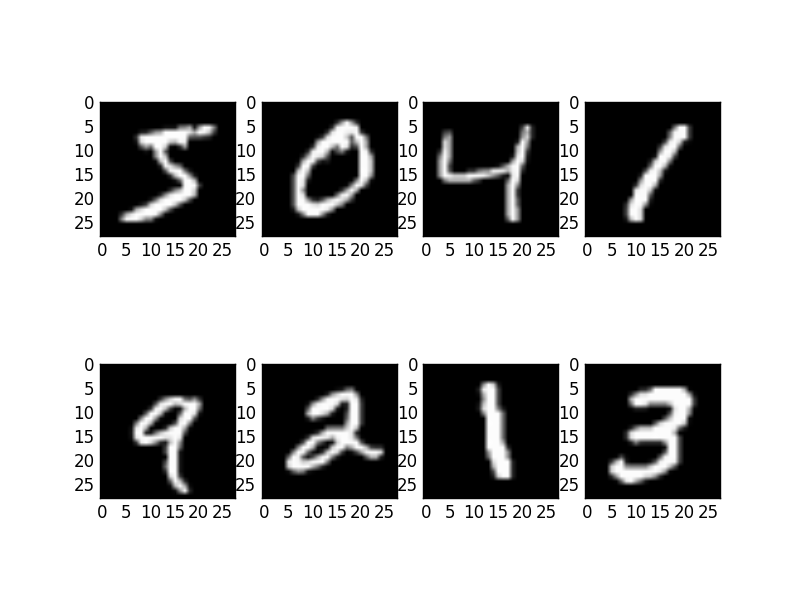
\includegraphics[width=12cm, keepaspectratio]{figures/mnist.png}
	\caption{Samples extracted from the MNIST database}
	\label{fig:mnist}
\end{figure}

\section{Keras}\label{sec:keras}
As stated by \textbf{Keras} documentation \cite{chollet2015keras}: "Keras is a high-level \textbf{neural network library}, written in Python and capable of running on top of either TensorFlow or Theano". TensorFlow and Theano are open-source libraries for numerical computation optimized for GPU and CPU that Keras treats as its \textit{backends}. In this project, Keras is running on top of \textbf{Theano} \footnote{\url{http://deeplearning.net/software/theano/index.html}} optimized for CPU, but it's quite easy to switch from one backend to another.

In the following sections, the main elements that make up a neural network built with Keras are going to be analyzed, starting with the \textbf{\textit{model} object}, its core component.

\subsection{Models}\label{subsec:models}
Every neural network in Keras is defined as a \textbf{\textit{model}}. For those models which can be built as a stack of \textit{layers} \ref{subsec:layers}, Keras provides the \textbf{\textit{.Sequential()} object}. An example of a sequential model built with Keras can be seen in figure \ref{fig:model}. It is also possible to build more complex models with multiple outputs and shared layers using the \textbf{Keras functional API}.
\begin{figure}
	\centering
	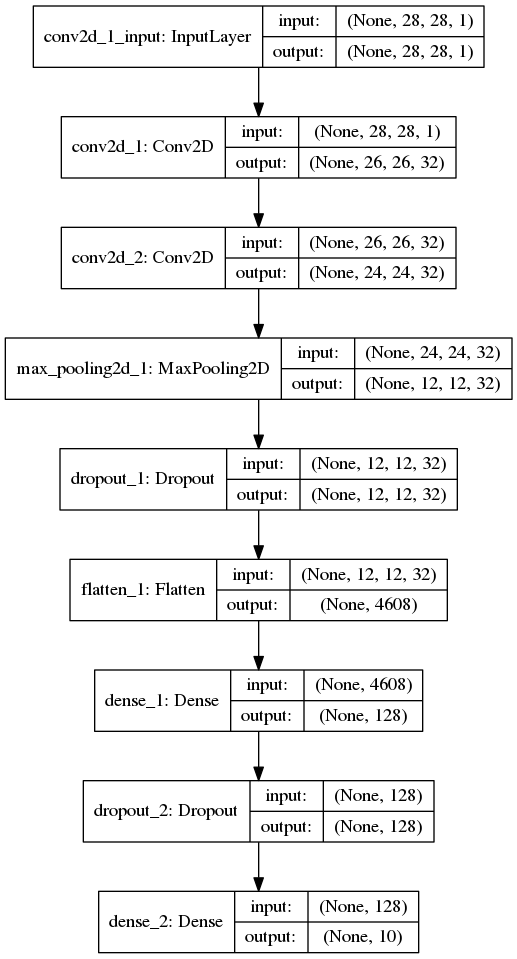
\includegraphics[width=8cm, keepaspectratio]{figures/model.png}
	\caption{Diagram of a Keras sequential model}
	\label{fig:model}
\end{figure}

Sequential models have several methods, and the following ones are essential for the learning process:
\begin{description}
	\item[\textit{.compile()}] It configures the learning process. It's main arguments are:
	\begin{itemize}
		\item \textbf{\textit{loss}}: name of the \textbf{cost function} employed to check the difference between the predicted label and the real one. In this project, the \textbf{categorical cross-entropy}, also known as log loss, has been used. It returns the cross-entropy between an approximating distribution $q$ and a true distribution $p$ \cite{2016arXiv160502688short} and it's defined as:
		\begin{equation}\label{eq:categorical_crossentropy}
		H(p,q)=-\Sigma_{x}p(x)\log(q(x))
		\end{equation}		
		Other loss functions such as mean squared error (MSE), mean absolute error and hinge are also provided by Keras.
		
		\item \textbf{\textit{optimizer}}: name of the optimizer that will update the weights values during training in order to minimize the value of the loss function. The chosen algorithm for this task is \textbf{ADADELTA} \cite{DBLP:journals/corr/abs-1212-5701}.
		
		Other optimization methods such as Adagrad, Adamax and Adam are also available.
		
		\item \textbf{\textit{metrics}}: name of the parameters that must be evaluated during training and testing. The only metric that is going to be calculated with Keras through this project, besides the result of the loss function which is automatically computed, is \textbf{accuracy}. It is defined as the proportion of examples for which the model produces the correct output \cite{Goodfellow-et-al-2016}.			
		Other metrics are calculated with \textbf{Scikit-learn} \ref{sec:sklearn} library, in order to obtain a evaluation of the model that is independent from Keras.
	\end{itemize}
\end{description}

\begin{description}
	\item[\textit{.fit()}] It trains the model. The following arguments are required:
	\begin{itemize}
		\item \textbf{\textit{x}, \textit{y}}: training samples and labels. They must be defined as \textbf{Numpy arrays}\footnote{\url{http://www.numpy.org/}}.
		
		\item \textbf{\textit{batch\_size}}: number of samples that are evaluated before updating the weights. It defaults to 32.
		
		\item \textbf{\textit{epochs}}: number of iterations over the whole dataset that are going to be executed. It defaults to 10.
		
		\item \textbf{\textit{callbacks}}: list of callbacks \ref{subsec:callbacks} that are going to be applied during training. It defaults to \textit{None}.
		
		\item \textbf{\textit{validation\_split} or \textit{validation\_data}}: On one hand, \textit{validation\_split} defines the fraction of the training data that has to be used as held-out validation data. On the other hand, \textit{validation\_data} is a tuple containing the samples and labels of a validation dataset provided by the user. They are mutually exclusive.
		
		\item \textbf{\textit{shuffle}}: a boolean that determines whether to shuffle training data or not. 
	\end{itemize}
\end{description}

\begin{description}
	\item[\textit{.evaluate()}] It takes a set of samples and labels and evaluates the \textbf{model performance}, returning a list of the metrics previously defined.
\end{description}

\begin{description}
	\item[\textit{.predict()}] It takes a sample and returns the label predicted by the model.
\end{description}

\begin{description}
	\item[\textit{.save()}] It stores the model into a \textbf{HDF5 file} \ref{sec:hdf}, which will contain the weights, architecture and training configuration of the model.
\end{description}

\begin{description}
	\item[\textit{.load\_model()}] It loads a model from a \textbf{HDF5 file}.
\end{description}

\subsection{Layers}\label{subsec:layers}
As it has been said before, the models are usually built as a \textbf{stack of layers}. These layers are added to the model using the \textbf{\textit{.add()} method}, inside of which the kind of layer is declared and its particular parameters are set. Several kinds of layers are available, but only the ones that have been used in this project are going to be described.
\begin{description}
	\item[Convolutional layer] This particular layer is the one that turns the neural network into a \textbf{convolutional neural network (CNN)}. It is formed by a fixed number of \textbf{filters/kernels} with a fixed size. These filters are convolved along the input image, generating each one a \textbf{feature or activation map} which will tell us to what extent the feature learned by that particular filter is present in the input image. Keras provides different kinds of convolutional layers depending on the input dimensions: \textit{Conv1D}, \textit{Conv2D} and \textit{Conv3D}. These are the main arguments required by Keras to define a convolutional layer:
	\begin{itemize}
		\item \textbf{\textit{filters}}: number of filters.
		
		\item \textbf{\textit{kernel\_size}}: width and height of the filters.
		
		\item \textbf{\textit{strides}}: how many pixels the filter must be shifted before applying the next convolution. Output size depends on this parameter. It defaults to 1.
		
		\item \textbf{\textit{padding}}: it can be \textit{valid} or \textit{same}. If \textit{valid} mode is set, no padding is applied, resulting in a reduced output. However, if \textit{same} mode is set, the input will be padded with zeros in order to produce an output that preserves the input size. It defaults to \textit{valid}.
	\end{itemize}
\end{description}

\begin{description}
	\item[{Pooling layer}] It shifts a window of a certain size along the input image applying an operation (mean or maximum) that will return a \textbf{\textit{downsampled} version} of it. Depending on the dimensions of the input and the operation applied, Keras provides several pooling layers: \textit{MaxPooling1D}, \textit{MaxPooling2D}, \textit{MaxPooling3D}, \textit{AveragePooling1D}... The main arguments required by Keras to define these layers are:
	\begin{itemize}
		\item \textbf{\textit{pool\_size}}: size of the window that is shifted along the input. It can also be interpreted as the factor by which the input is going to be downsampled.
		\item \textbf{\textit{strides}}: how many pixels the window must be shifted before applying the next operation.
	\end{itemize}
\end{description}

\begin{description}
	\item[Dense layer] Fully-connected layers in Keras are defined as \textit{Dense layers}. In a \textbf{fully-connected layer}, every neuron is connected to every activation (output) of the previous one. The main argument of this layer is:
	\begin{itemize}
		\item \textbf{\textit{units}}: number of neurons.
	\end{itemize} 
\end{description}

\begin{description}
	\item[Activation layers] In Keras models, activations can be declared as a layer itself, or as an argument within the \textit{.add()} method of the previous layer. Keras provides several \textbf{activation functions}, such as sigmoid, linear, ReLU and softmax. The only argument that must be provided to activation layers is the name of the desired activation function. These are the ones that have been used during the development of this project:
	\begin{itemize}
		\item \textbf{ReLU (Rectified Linear Unit)}: This activation function introduces \textbf{non-linearity} right after each convolutional layer, allowing the CNN to learn more complex features. It's defined as:
		\begin{equation}\label{eq:ReLU}
		g(z)=\max(0,z)
		\end{equation}
		
		\item \textbf{Softmax} This activation function is very useful when is placed after the \textbf{output layer} of classification tasks. It takes a vector of real values $z$ and returns a new vector of real values in the range [0,1]. The $N$ elements of the output vector can be considered \textbf{probabilities} because the softmax function ensures that they sum up to 1. It is defined as follows:
		\begin{equation}\label{eq:SoftMax}
		\mathrm{softmax}(z)_i=\frac{\exp(z_i)}{\Sigma_{j}{\exp(z_j)}} \quad \mathrm{for} \ j=1, ...,N
		\end{equation}
	\end{itemize}
	These equations \cite{Goodfellow-et-al-2016} are equivalent to the ones employed by Keras, defined by its backends: Theano and Tensorflow.
\end{description}

\begin{description}
	\item[Flatten layer] It \textit{flattens} the input. For instance, it converts the activation maps returned by the convolutional layers into a \textbf{vector of neurons} before being connected to a dense layer. It takes no arguments.
\end{description}

\begin{description}
	\item[Dropout layer] It's considered a \textbf{regularization layer}, because its main purpose is to avoid over-fitting. Dropout \cite{Srivastava-et-al-2014} is a technique that randomly \textbf{\textit{switches-off}} a fraction of hidden units during training, both forward and backward propagation. This layer, as other regularization layers (i.e. GaussianNoise layer), is only active during training. It's main argument is:
	\begin{itemize}
		\item \textbf{\textit{rate}}: fraction of units that must be dropped.
	\end{itemize}
\end{description}

\subsection{Callbacks} \label{subsec:callbacks}
As defined by Keras documentation \cite{chollet2015keras}, \textbf{callbacks} are a set of functions which are applied at given stages while the model is being trained. They can be used to take a look at the state of the model during training. The built-in callbacks that have been used for this project are:
\begin{itemize}
	\item \textbf{\textit{.History()}}: it is automatically applied to every Keras model and is returned by the \textit{.fit()} method. It evaluates the declared metrics with the validation set after each epoch and saves the results.
	
	\item \textbf{\textit{.EarlyStopping()}}: it monitors the value of a given metric and forces the model to stop training when that metric has stopped improving. It has a \textbf{\textit{patience}} argument which determines how many epochs in a row without improving must be tolerated before the model quits training. Setting up an appropriate \textbf{stopping criteria} may prevent the model from over-fitting.
	
	\item \textbf{\textit{.ModelCheckpoint()}}: it saves the model and its weights after each epoch. It can be configured to overwrite the model only if a certain metric has improved with respect to the previous best result, saving the best \textit{version} of it.
\end{itemize}

Additionally, Keras provides the \textit{Callback} base class that can be used to build \textbf{user-defined callbacks}.

\subsection{Image Preprocessing}
\textbf{Image preprocessing} is a key factor in every computer vision application. Specifically, in machine learning, besides adapting the image and extracting features before the training that can improve the model performance (i.e. edge extraction), it can be used to avoid \textbf{over-fitting} through data augmentation. \textbf{Data augmentation} consists in taking the samples that the dataset already contains and applying transformations to them, generating new samples that may be closer to real world and, in any case, enlarging the dataset with new data.

This functionality is included in Keras thanks to the \textbf{\textit{.ImageDataGenerator()} method}. It returns a batch generator which randomly applies the desired \textbf{transformations} to random samples of the dataset provided by the user. Built-in transformations like rotation, shifting and zooming, are passed as arguments to the aforementioned method. Additionally, it's possible to build a user-defined function and pass it as an argument as well. The dataset, and the batch size are defined through the \textbf{\textit{.flow()} method}. During training, the generator will loop until the number of samples per epoch and the number of epochs set by the user are satisfied.

\subsection{Utils}
Keras include a module for multiple supplementary tasks called \textbf{\textit{Utils}}. The most important functionality for the project provided by this module is the \textbf{\textit{.HDF5Matrix()} method}. It reads the \textbf{HDF5 datasets} \ref{sec:hdf}, which are going to be used as inputs to the neural networks.

\section{HDF5}\label{sec:hdf}
During the development of this project, \textbf{huge amounts of data} have been processed. That's why an efficient way of reading and saving this data has been an important point. Keras employs the \textbf{HDF5 file format} to save models and read datasets.

According to HDF5 (Hierarchical Data Format) documentation \cite{hdf5}, it is designed for high volumes of data with complex relationships. While relational databases employ tables to store data, HDF5 supports \textbf{n-dimensional datasets} and each element in the dataset may be as complex as needed.

In order to deal with HDF5 files, the \textbf{h5py} \footnote{\url{http://www.h5py.org/}} library for Python has been employed.

\section{Scikit-learn}\label{sec:sklearn}
\textbf{Scikit-learn} \cite{scikit-learn} is a \textbf{machine learning library} that includes a wide variety of algorithms for clustering, regression and classification. It can be used during the whole machine learning process: preprocessing, training, model selection and evaluation.

Scikit-learn functions have been used to evaluate the neural networks developed with Keras. Using a tool that is \textbf{independent from Keras} enables the comparison of the results achieved by different neural network libraries (e.g. Keras and Caffe). These are the \textbf{metrics} employed in this project:
\begin{itemize}
	\item \textbf{Precision}: ability of the classifier not to label as positive a sample that is negative.
	\begin{equation}\label{eq:precision}
	\textrm{precision}=\frac{true_{positives}}{true_{positives}+false_{positives}}
	\end{equation}
	
	\item \textbf{Recall}: ability of the classifier to find all the positive samples.
	\begin{equation}\label{eq:recall}
	\textrm{recall}=\frac{true_{positives}}{true_{positives}+false_{negatives}}
	\end{equation}
	
	\item \textbf{Confusion matrix}: a matrix where the element $i,j$ represents the number of samples that belongs to the group $i$ but has been classified as belonging to group $j$. True predictions can be found in the diagonal of the matrix, where $i=j$. An example of a confusion matrix constructed with Scikit-learn and displayed with Octave \ref{sec:octave} can be found in figure \ref{fig:conf_mat}.
\end{itemize}

Besides the metrics that have just been mentioned, \textbf{accuracy} and \textbf{log loss} have also been used and they're defined as in section \ref{subsec:models}.

\section{Octave} \label{sec:octave}
\textbf{GNU Octave} \footnote{\url{https://www.gnu.org/software/octave/}} is a scientific programming language compatible with \textbf{Matlab}. It provides powerful tools for \textbf{plotting}, which have been used to visualize the data collected with Scikit-learn about the performance of the models. An example of Octave usage can be seen in the figure \ref{fig:conf_mat}.
\begin{figure}
	\centering
	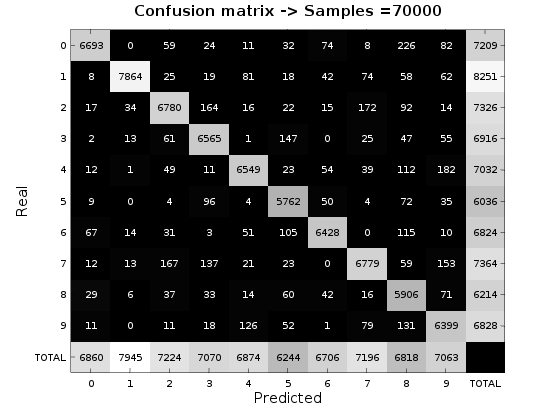
\includegraphics[width=12cm, keepaspectratio]{figures/conf_mat.png}
	\caption{Example of a confusion matrix visualization using Octave}
	\label{fig:conf_mat}
\end{figure}